
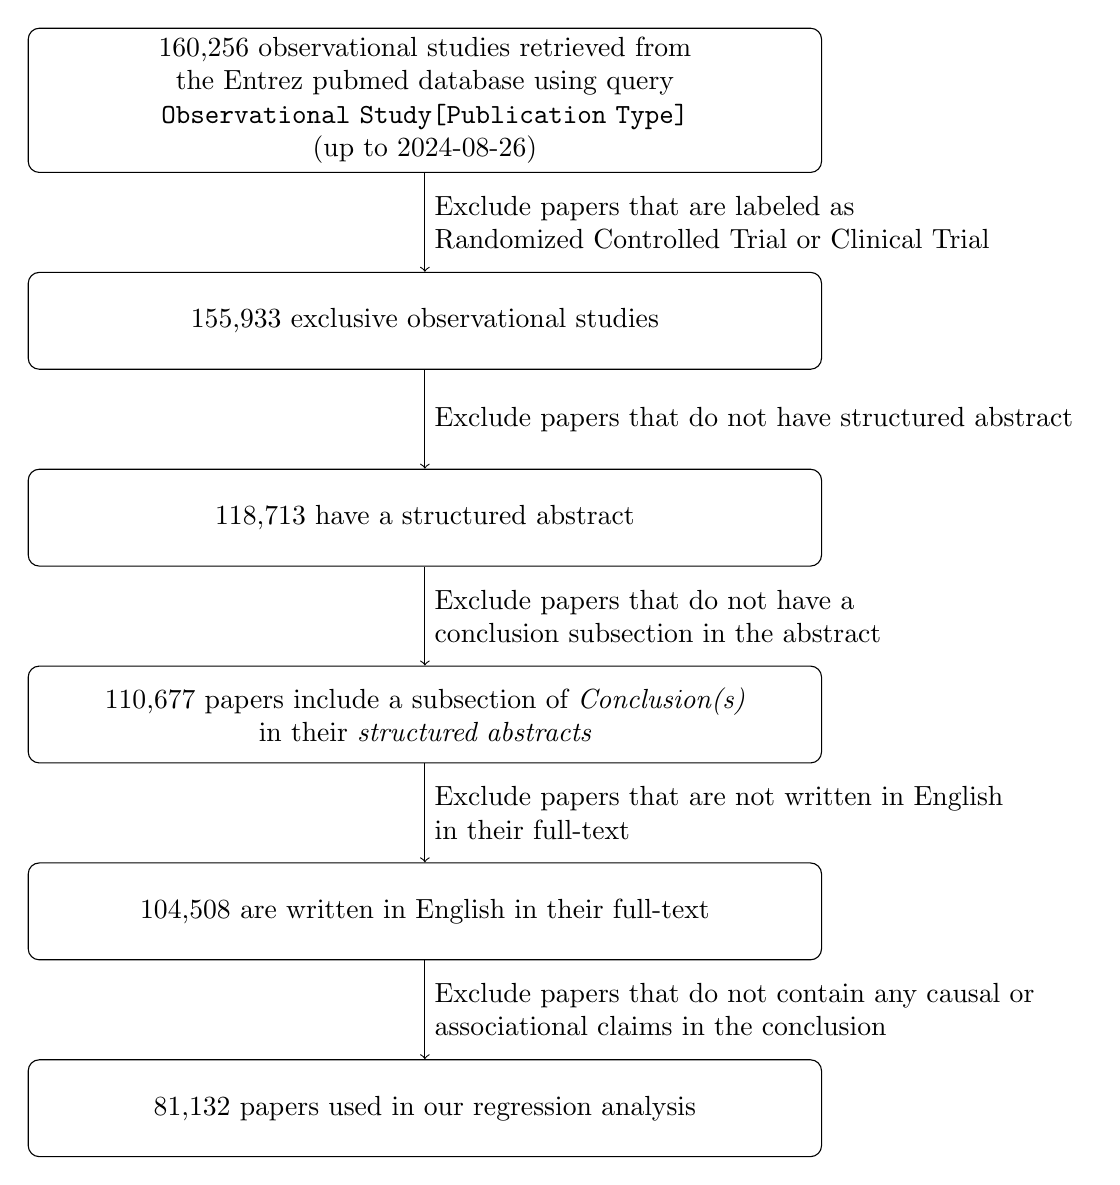
\begin{tikzpicture}
    \tikzstyle{block} = [rectangle, rounded corners, draw, text width=28em, text centered, minimum height=3.5em]

    % Place nodes
    \node [block] (block1) {160,256 observational studies retrieved from the Entrez pubmed database
    using query {\tt Observational Study[Publication Type]} \\
    (up to 2024-08-26)};
    
    \node [block, below of=block1, yshift=-1.8cm] (block2) {
        155,933 exclusive observational studies
    };
    
    \node [block, below of=block2, yshift=-1.5cm] (block2_3) {
        118,713 have a structured abstract \\ 
    };
    \node [block, below of=block2_3, yshift=-1.5cm] (block3) {
        110,677 papers include a subsection of {\em Conclusion(s)} \\ in their {\em structured abstracts}
    };
    \node [block, below of=block3, yshift=-1.5cm] (block4) {
        104,508 are written in English in their full-text
    };
    \node [block, below of=block4, yshift=-1.5cm] (block5) {
        81,132 papers used in our regression analysis
    };

    \draw[->] (block1) -- (block2) node[anchor=west, midway, align=left] {
        Exclude papers that are labeled as \\ Randomized Controlled Trial or Clinical Trial
    };
    
    \draw[->] (block2) -- (block2_3) node[anchor=west, midway, align=left] {
        Exclude papers that do not have structured abstract 
    };

    \draw[->] (block2_3) -- (block3) node[anchor=west, midway, align=left] {
        Exclude papers that do not have a \\ conclusion subsection in the abstract
    };

    \draw[->] (block3) -- (block4) node[anchor=west, midway, align=left] {
        Exclude papers that are not written in English \\ in their full-text
    };

    \draw[->] (block4) -- (block5) node[anchor=west, midway, align=left] {
        Exclude papers that do not contain any causal or \\
        associational claims in the conclusion 
    };

\end{tikzpicture}
